\documentclass[12pt]{article}

\usepackage{listings}
\renewcommand{\lstlistingname}{Code}
\usepackage{xcolor}
\lstdefinestyle{sharpc}{language=[Sharp]C, frame=lr, rulecolor=\color{blue!80!black}}
\usepackage{graphicx}
\usepackage[style=authoryear]{biblatex}
\usepackage{setspace}
\addbibresource{references.bib}
\onehalfspacing

\begin{document}

\begin{titlepage}
	\centering
	
	%opening
	\title{Gamification of Gaussian Splats \\ {\large Rendering and Animating multiple Gaussian Splats in a Unity scene}}
	
	\author{Bavo Verstraeten}
	
	
	
	\maketitle
\end{titlepage}
	
\begin{abstract}
Gaussian splatting has emerged as a powerful technique for real-time rendering of complex 3D scenes. While existing implementations focus on efficient rendering, their integration into interactive applications such as games remains underexplored. This thesis investigates the gamification of Gaussian Splats in Unity, enabling multiple Gaussian Splat GameObjects to coexist within a scene, each with its own transform and animation. A key challenge is ensuring correct rendering while maintaining real-time performance. A current popular approach, a widely used Unity extension, processes splats in a per-GameObject order rather than achieving a globally correct sorting of individual splats. This work aims to overcome these limitations by adapting its rendering pipeline.
\end{abstract}

\begin{titlepage}
\centering
\tableofcontents
\end{titlepage}
\section{Background}
\subsection{From Meshes to Gaussian Splatting}
\subsubsection{Triangle Meshes}
In the field of computer graphics, the efficient rendering of complex 3D scenes has consistently posed a significant challenge. Traditional rendering techniques predominantly rely on triangle meshes, where the representation of surfaces is approximated through a network of interconnected triangles. While these methods have proven effective in many applications, they encounter limitations when dealing with highly detailed or non-uniform data. Achieving photorealistic results in such cases necessitates considerable memory and computational resources. Furthermore, these approaches are heavily dependent on manually crafted 3D models, a process that is both time-consuming and requires skilled artist. The generation of models from video or a collection of images offers the potential for a significantly simpler and more scalable solution.
\begin{figure}[h!]
	\centering
	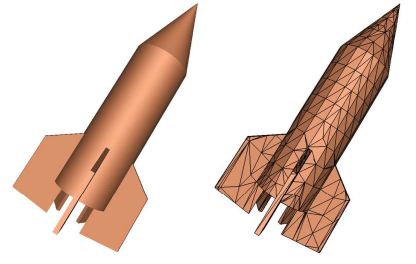
\includegraphics[width=\textwidth]{Images/TriangleMesh.png}
	\caption{Example of a triangle mesh, the most commonly used method for representing 3D objects in computer graphics. Image is taken from \cite{Mesh}}
	\label{fig:trianglemesh}
\end{figure}
\newpage
\subsubsection{Neural Radiance Fields}
One popular approach to addressing these challenges is Neural Radiance Fields (NeRF) \parencite{Nerf}, introduced in 2020. This method employs a neural network to learn a mapping from 3D position and viewing direction to an RGB color and density. The network is trained on a video or a collection of images, allowing it to reconstruct a scene by learning the underlying volumetric representation. During rendering, a ray is cast through each pixel of the screen, and multiple points along the ray are sampled. The neural network takes the position of each point and the viewing direction of the ray as input, producing color and density values. These outputs are then aggregated to compute the final color of the pixel, enabling the generation of photorealistic scenes without the need for manually crafted 3D models. However, due to the necessity of querying the neural network multiple times per pixel, this approach is computationally expensive and not suitable for real-time rendering.
\begin{figure}[h!]
	\centering
	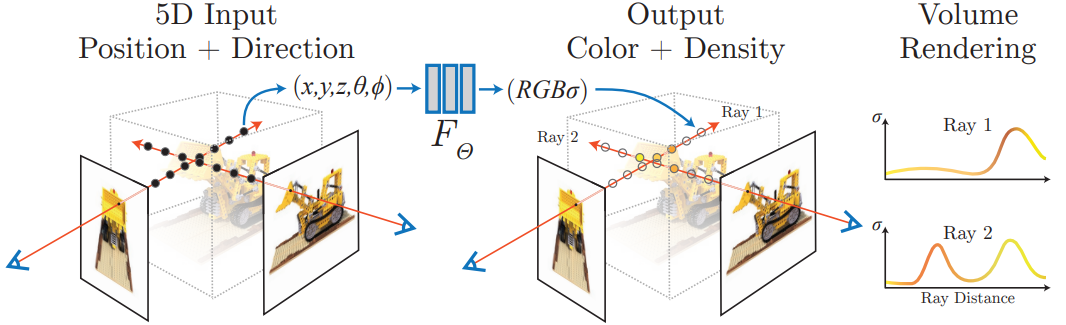
\includegraphics[width=\textwidth]{Images/Nerf.png}
	\caption{Rendering a scene using Neural Radiance Fields. Image is taken from \cite{Nerf}}
	\label{fig:nerf}
\end{figure}
\subsubsection{Gaussian Splatting}
In 2023, a method was introduced that retained the advantages of Neural Radiance Fields, while achieving real-time processing: Gaussian Splatting \parencite{OriginalSplatting}. Like Neural Radiance Fields, Gaussian Splatting uses a video or a collection of images as input to automatically generate the 3D scene data. However, rather than relying on a neural network to represent the data, the scene is represented as a collection of numerous small 3D Gaussians.
\begin{figure}[h!]
	\centering
	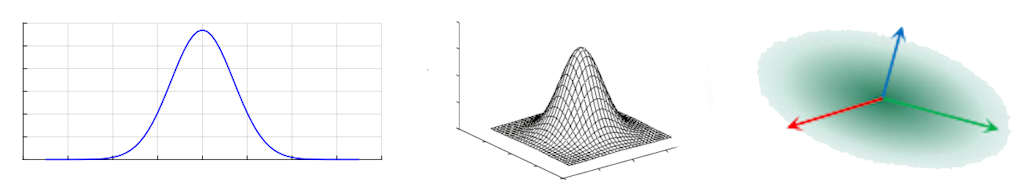
\includegraphics[width=\textwidth]{Images/GaussianForm.png}
	\caption{Illustration of Gaussian functions in different dimensions, shown left to right: 1D Gaussian \parencite{1DGaussian}, 2D Gaussian \parencite{2DGaussian}, and 3D Gaussian \parencite{3DGaussian}}
	\label{fig:Form}
\end{figure}
\newpage  \noindent
Each Gaussian is defined by several attributes that determine its appearance and behavior during rendering:
\begin{itemize}
	\item 3D coordinates
	\item Opacity (transparency)
	\item Anisotropic covariance: The degree to which the Gaussian is 'stretched' along each of the three axes independently
	\item Spherical Harmonics: The color of the Gaussian, which varies depending on the viewing angle
\end{itemize}
The key advantage of this approach is the way the scene is rendered. Instead of relying on rays or neural networks, which are computationally expensive, Gaussian Splatting leverages a rasterization technique. In this process, the 3D Gaussians are projected directly onto the 2D screen space, where they are rendered as small, disk-like splats (when this paper refers to 'splats', it means one such disk-like object). These splats are then blended together based on their spatial overlap, opacity, and color attributes.\\
Furthermore, state-of-the-art triangle mesh rendering also relies on rasterization, meaning that this approach already benefits from many well-established optimizations in graphics hardware. These optimizations, including efficient handling of spatial data and parallel processing, are directly applicable to Gaussian Splatting. By utilizing the same rendering pipeline, Gaussian Splatting can leverage these optimizations for further efficiency gains, making it an ideal choice for real-time rendering applications.
\subsection{Unity Extension}
\subsubsection{Introduction}
When it comes to the gamification of this technique, multiple engines come to mind, such as Unity, Godot, and Unreal Engine. Among these, Unity was chosen due to prior experience with the engine. Additionally, a widely referenced GitHub project \parencite{Aras} implementing Gaussian Splatting in Unity provides a strong foundation for further research. This project stands out not only for its recognition within the community \parencite{ArasRecc1} \parencite{ArasRecc2}, but also for its developer, Aras Pranckevičius, a former Unity engineer with 15 years of experience working on the engine. His expertise suggests that the rendering pipeline adaptations are both well-optimized and efficiently integrated, making this implementation a suitable choice for exploration and development.
\\\\
Before examining the objectives of this thesis and the adaptations made to the selected implementation, it is essential to first outline the relevant aspects of its rendering pipeline. The discussion will focus solely on components that directly influence the rendering process. Certain aspects, such as the compression and storage of Gaussian Splats in files, among others, fall outside the scope of this explanation and will not be covered.
\subsubsection{Adding a Gaussian Splat to the Scene}
The selected project does not implement the training of Gaussian Splats but instead relies on pretrained models obtained from an external source. These models are not used in their original format; rather, the project includes a Unity Editor extension that converts them into a more efficient and compressed representation. As previously mentioned, the specifics of this compression process have minimal impact on rendering and will therefore not be discussed in detail. Once the compressed asset is generated, the user must manually create a new empty GameObject and attach the \texttt{GaussianSplatRenderer} script to it. This script includes a field labeled Asset, into which the compressed asset must be assigned. Upon doing so, the Gaussian Splat appears in the scene. Like any GameObject in Unity, it can be translated, rotated, and scaled. This process can be repeated to instantiate multiple Gaussian Splats within the same scene.
\begin{figure}[h!]
	\centering
	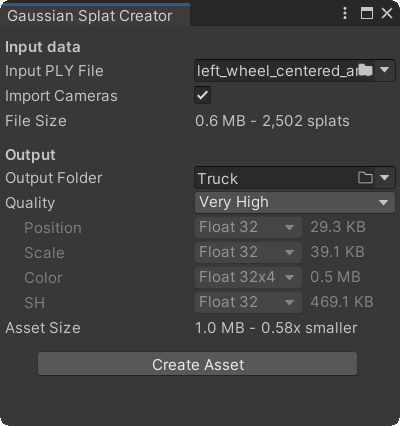
\includegraphics[width=0.5\textwidth]{Images/SplatCreator.png}
	\caption{The Unity Editor extension included in the project for converting PLY files into the required compressed format}
	\label{fig:creator}
\end{figure}
\subsubsection{Initializing the Rendering Process: The Role of \texttt{OnEnable}}
When no GameObjects with an attached \texttt{GaussianSplatRenderer} script are present, the renderer follows the standard rendering pipeline. However, once such a GameObject is enabled, its \texttt{OnEnable} method is executed, performing several initialization tasks. The method is outlined in the following code snippet:
\lstset{style=sharpc}
\begin{lstlisting}[tabsize=2,caption=\texttt{onEnable} of \texttt{GaussianSplatRenderer}, label=code:rendereronenable,breaklines=true,breakatwhitespace=true,basicstyle=\ttfamily\footnotesize]
public void OnEnable()
{
  // Check if necessary shaders and compute shaders are available

	// Initialize materials (details omitted, see later)
	
	// Initialize the sorter
	
	GaussianSplatRenderSystem.instance.RegisterSplat(this);
	
	// Initialize all the graphics buffers
}
\end{lstlisting}
As demonstrated in the code segment, the \texttt{OnEnable} method calls the \linebreak\texttt{RegisterSplat} function of \texttt{GaussianSplatRenderSystem}, a singleton class. This class plays a pivotal role in managing the multiple \linebreak\texttt{GaussianSplatRenderer} objects within the scene and is responsible for executing the changes that modify the rendering process. The implementation of the \texttt{RegisterSplat} function is as follows:
\begin{lstlisting}[tabsize=2,caption=\texttt{RegisterSplat} of \texttt{GaussianSplatRenderSystem}, label=code:systemregister,breaklines=true,breakatwhitespace=true,basicstyle=\ttfamily\footnotesize]
public void RegisterSplat(GaussianSplatRenderer r)
{
	if (m_Splats.Count == 0)
	{
		if (GraphicsSettings.currentRenderPipeline == null)
		Camera.onPreCull += OnPreCullCamera;
	}
	m_Splats.Add(r, new MaterialPropertyBlock());
}
\end{lstlisting}
The \texttt{GaussianSplatRenderSystem} maintains a dictionary of all enabled \linebreak\texttt{GaussianSplatRenderer} objects. When this function is invoked, and no other \texttt{GaussianSplatRenderer} are registered, the method subscribes to the \texttt{Camera.onPreCull} event, linking it to the \texttt{OnPreCullCamera} method.\\
When a \texttt{GaussianSplatRenderer} is disabled, it clears all associated buffers and materials, removes the object from the internal dictionary, and unsubscribes from the \texttt{onPreCull} event when the last \texttt{GaussianSplatRenderer} is removed, effectively managing resources and maintaining system efficiency.
\subsubsection{The Rendering Pipeline}
Each frame, the Unity engine performs culling before rendering the scene, determining which objects lie within the camera’s view and should be processed for rendering. Since splats may appear outside of the camera’s view, the moment just prior to culling is an optimal point at which to prepare these splats and enqueue their draw procedure in the command buffer for execution during the rendering stage. That moment is when \texttt{onPreCull} calls are made.\\
As previously mentioned, when the first \texttt{GaussianSplatRenderer} is enabled, the \texttt{OnPreCullCamera} function is linked to \texttt{onPreCull}. The implementation of this function is as follows:
\begin{lstlisting}[tabsize=2,caption=\texttt{OnPreCullCamera} of \texttt{GaussianSplatRenderSystem}, label=code:systemprecull,breaklines=true,breakatwhitespace=true,basicstyle=\ttfamily\footnotesize]
void OnPreCullCamera(Camera cam)
{
	if (!GatherSplatsForCamera(cam))
	return;
	
	InitialClearCmdBuffer(cam);
	
	m_CommandBuffer.GetTemporaryRT( GaussianSplatRenderer.Props.GaussianSplatRT, -1, -1, 0, FilterMode.Point, GraphicsFormat.R16G16B16A16_SFloat);
	m_CommandBuffer.SetRenderTarget( GaussianSplatRenderer.Props.GaussianSplatRT, BuiltinRenderTextureType.CurrentActive);
	m_CommandBuffer.ClearRenderTarget(RTClearFlags.Color, new Color(0, 0, 0, 0), 0, 0);
	
	// add sorting, view calc and drawing commands for each splat object
	Material matComposite = SortAndRenderSplats(cam, m_CommandBuffer);
	
	// compose
	m_CommandBuffer.BeginSample(s_ProfCompose);
	m_CommandBuffer.SetRenderTarget( BuiltinRenderTextureType.CameraTarget);
	m_CommandBuffer.DrawProcedural(Matrix4x4.identity, matComposite, 0, MeshTopology.Triangles, 3, 1);
	m_CommandBuffer.EndSample(s_ProfCompose);
	m_CommandBuffer.ReleaseTemporaryRT( GaussianSplatRenderer.Props.GaussianSplatRT);
}
\end{lstlisting}
This function performs 5 key operations:
\begin{itemize}
	\item \texttt{GatherSplatsForCamera}: This function first iterates over all key-value pairs in \texttt{m\textunderscore Splats} and selects those that have a valid compressed asset assigned, storing them in the list \texttt{m\textunderscore ActiveSplats}. Subsequently, this list is sorted based on the depth of each entry’s transform in the camera’s coordinate space. The implementation of this function will be presented later.
	\item \texttt{InitialClearCmdBuffer}: This function initializes and clears a command buffer, \texttt{m\textunderscore CommandBuffer}, before attaching it to the camera. By doing so, draw commands, which are created in later parts of the code, can be enqueued into this buffer. Each draw command ensures execution during the later rendering process if it is not culled.
	\item The function creates a temporary render target, \texttt{GaussianSplatRT}, sets it as the active render target, and clears it. Consequently, any draw calls issued before the render target is switched again will render to this temporary target rather than directly to the camera’s output.
	\item \texttt{SortAndRenderSplats}: This function is responsible for the main calculations. It processes all collected splats and enqueues the necessary draw commands to render them into \texttt{GaussianSplatRT}. The implementation of this function will be presented later.
	\item  The render target is reset to the camera’s primary output, after which a \texttt{DrawProcedural} call is issued using a designated material. This material is associated with a shader that generates a  single triangle that covers the entire screen in its vertex shader. The fragment shader subsequently reads data from \texttt{GaussianSplatRT} and applies gamma correction. This \texttt{DrawProcedural} call enqueues the rendering of this full-screen triangle, ensuring that the Gaussian Splats are correctly displayed in the final rendered image.
\end{itemize}
To fully understand what gets rendered to the screen, it is essential to take a close look at \texttt{SortAndRenderSplats}:
\begin{lstlisting}[tabsize=2,caption=\texttt{SortAndRenderSplats} of \texttt{GaussianSplatRenderSystem}, label=code:systemsortrender,breaklines=true,breakatwhitespace=true,basicstyle=\ttfamily\footnotesize]
public Material SortAndRenderSplats(Camera cam, CommandBuffer cmb)
{
	Material matComposite = null;
	foreach (var kvp in m_ActiveSplats)
	{
		var gs = kvp.Item1;
		matComposite = gs.m_MatComposite;
		var mpb = kvp.Item2;
		
		// sort
		var matrix = gs.transform.localToWorldMatrix;
		if (gs.m_FrameCounter % gs.m_SortNthFrame == 0)
		gs.SortPoints(cmb, cam, matrix);
		++gs.m_FrameCounter;
		
		kvp.Item2.Clear();
		Material displayMat = gs.m_RenderMode switch
		{
			GaussianSplatRenderer.RenderMode.DebugPoints => gs.m_MatDebugPoints,
			GaussianSplatRenderer.RenderMode.DebugPointIndices => gs.m_MatDebugPoints,
			GaussianSplatRenderer.RenderMode.DebugBoxes => gs.m_MatDebugBoxes,
			GaussianSplatRenderer.RenderMode.DebugChunkBounds => gs.m_MatDebugBoxes,
			_ => gs.m_MatSplats
		};
		if (displayMat == null)
		continue;
		
		gs.SetAssetDataOnMaterial(mpb);
		mpb.SetBuffer(GaussianSplatRenderer.Props.SplatChunks, gs.m_GpuChunks);
		
		mpb.SetBuffer(GaussianSplatRenderer.Props.SplatViewData, gs.m_GpuView);
		
		mpb.SetBuffer(GaussianSplatRenderer.Props.OrderBuffer, gs.m_GpuSortKeys);
		mpb.SetFloat(GaussianSplatRenderer.Props.SplatScale, gs.m_SplatScale);
		mpb.SetFloat(GaussianSplatRenderer.Props.SplatOpacityScale, gs.m_OpacityScale);
		mpb.SetFloat(GaussianSplatRenderer.Props.SplatSize, gs.m_PointDisplaySize);
		mpb.SetInteger(GaussianSplatRenderer.Props.SHOrder, gs.m_SHOrder);
		mpb.SetInteger(GaussianSplatRenderer.Props.SHOnly, gs.m_SHOnly ? 1 : 0);
		mpb.SetInteger(GaussianSplatRenderer.Props.DisplayIndex, gs.m_RenderMode == GaussianSplatRenderer.RenderMode.DebugPointIndices ? 1 : 0);
		mpb.SetInteger(GaussianSplatRenderer.Props.DisplayChunks, gs.m_RenderMode == GaussianSplatRenderer.RenderMode.DebugChunkBounds ? 1 : 0);
		
		cmb.BeginSample(s_ProfCalcView);
		gs.CalcViewData(cmb, cam, matrix);
		cmb.EndSample(s_ProfCalcView);
		
		// draw
		int indexCount = 6;
		int instanceCount = gs.splatCount;
		MeshTopology topology = MeshTopology.Triangles;
		if (gs.m_RenderMode is GaussianSplatRenderer.RenderMode.DebugBoxes or GaussianSplatRenderer.RenderMode.DebugChunkBounds)
		indexCount = 36;
		if (gs.m_RenderMode == GaussianSplatRenderer.RenderMode.DebugChunkBounds)
		instanceCount = gs.m_GpuChunksValid ? gs.m_GpuChunks.count : 0;
		
		cmb.BeginSample(s_ProfDraw);
		cmb.DrawProcedural(gs.m_GpuIndexBuffer, matrix, displayMat, 0, topology, indexCount, instanceCount, mpb);
		cmb.EndSample(s_ProfDraw);
	}
	return matComposite;
}
\end{lstlisting}
This code block is extensive and encompasses multiple operations. To facilitate a clearer understanding, we will analyze it step by step, breaking it down into its fundamental components. Additionally, certain sections of the code are dedicated to debugging or timing purposes, which are not essential for understanding the main rendering pipeline.\\\\
The function iterates over all \texttt{GaussianSplatRenderer} objects stored and ordered in the \texttt{m\textunderscore ActiveSplats} list by \texttt{GatherSplatsForCamera}. It is important to emphasize that within this function, all subsequent operations are performed on a single \texttt{GaussianSplatRenderer} object at a time, as each iteration of the loop processes one individual \texttt{GaussianSplatRenderer}.\\\\
At regular intervals, specifically every set number of frames, the splats undergo sorting. This operation is managed by a custom sorter class, which was initialized during the \texttt{OnEnable} method. The class implements a specialized sorting algorithm known as "Device Radix Sort," leveraging the full potential of the GPU to ensure optimal performance. According to the comments in that class, this algorithm was adapted from another GitHub project \parencite{Sorting}. As with the sorting of the \texttt{GaussianSplatRenderer} objects, the depth of each splat relative to the camera’s coordinate space is used as the key for sorting.
\\\\
Similar to the final \texttt{DrawProcedural} invocation of the previous function, a material shader is employed at the end of each iteration of the loop to render the splats. Many of the operations within this loop are dedicated to populating graphics buffers with the necessary data for these shader computations. The most significant step in this process is the invocation of \texttt{CalcViewData}, This shader determines the screen-space position of each splat, calculates its independent horizontal and vertical extents, and derives its color and transparency based on the viewing angle and spherical harmonics. The computed results are then stored in a graphics buffer for subsequent use, \\\\
Finally, \texttt{DrawProcedural} is called, enqueueing the rendering of this data for execution later in the rendering pipeline. As before, this rendering is performed using a material shader, a different one from the material shader discussed earlier. Each splat is represented as two triangles, with the vertex shader transforming the computed screen position and stretch extents into appropriate triangle coordinates.
\\\\
As a brief reminder, as stated earlier, this \texttt{DrawProcedural} invocation does not render directly to the camera’s output but instead to the temporary render target \texttt{GaussianSplatRT}. Additionally, due to the sorting performed at the beginning of the loop, splats farther from the camera are rendered before those closer to it, ensuring correct per-object rendering order.
\section{Experiments and Development}
\subsection{Preparing the scene}
\subsection{Initial Workarounds and Approximate Solutions}
\subsection{Towards a Correct Rendering Pipeline}

\addcontentsline{toc}{section}{References}
\printbibliography
\end{document}
